\subsection*{Resultater}
Resultater har en boundary, hvortil der er opstillet en controlklasse. Boundary og tilhørende controller fremgår af \autoref{fig:MVCresultater}. 

\begin{figure} [H]
\centering
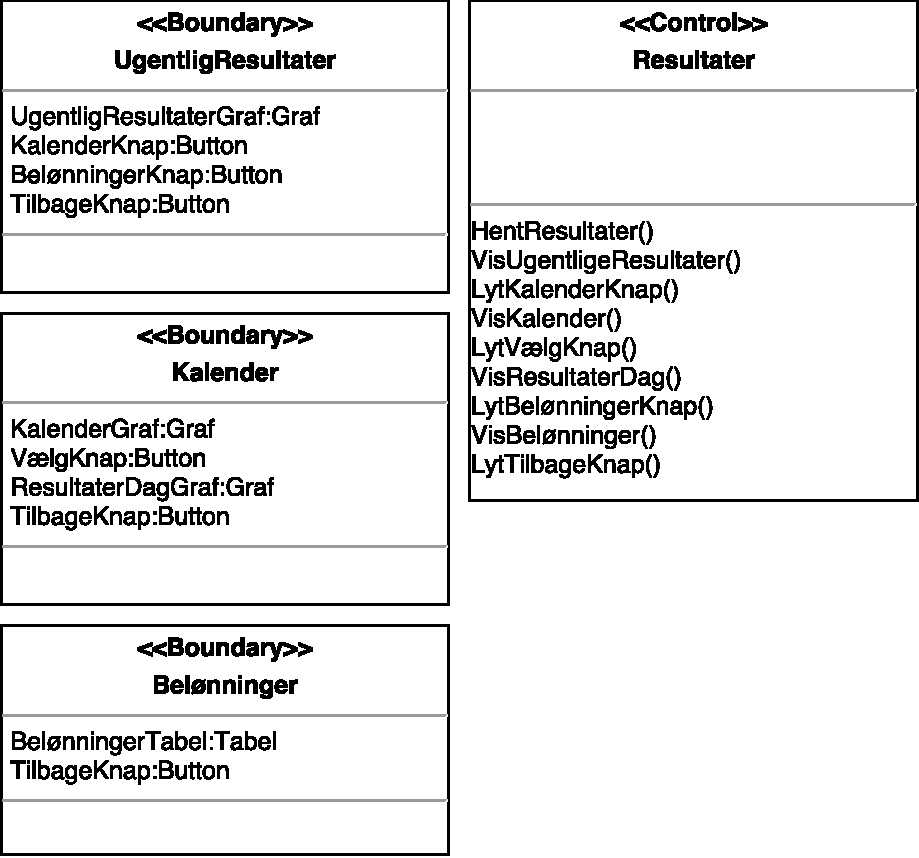
\includegraphics[width=0.5\textwidth]{figures/MVC/MVCResultater}
\caption{Designklasser for resultater. Til venstre ses boundary for Belønninger. Til højre fremgår den tilhørende controller.}
\label{fig:MVCresultater}
\end{figure}

\noindent
I grænsefladen image af typen ImageView og tekstfelter af typen TextView. Billederne viser antallet af stjerner, brugeren har opnået.
Controlleren for \textit{Resultater} indeholder Hent, Vis, Lyt og Start-metoder. 

I sammenspil med designklasserne for resultater er der udarbejdet et sekvensdiagram, hvilket fremgår af \autoref{fig:SEKResultater}

\begin{figure} [H]
\centering
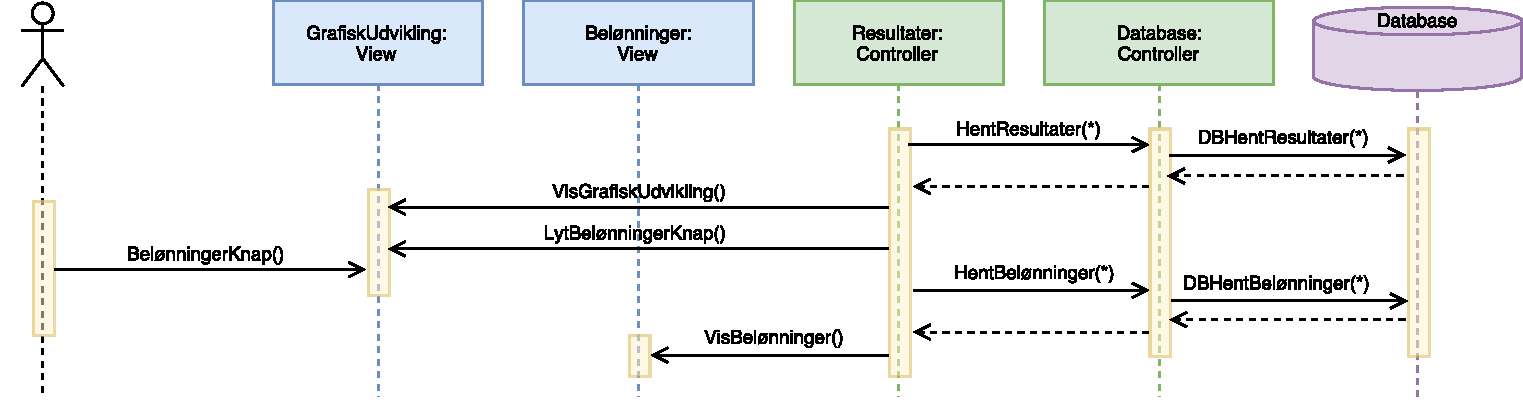
\includegraphics[width=1\textwidth]{figures/Sek/SEKResultater}
\caption{Sekvensdiagram for Resultater.}
\label{fig:SEKResultater}
\end{figure} 

\noindent 
Når brugeren er tilgået resultater henter controlleren, \textit{KonditionResultater} resultater fra \textit{Databasen} via dens controller. Hvis brugeren endnu ikke har nogle resultater, vil disse ikke hentes, hvorved disse ikke vil vises i grænsefladen for \textit{Belønninger}. Grænsefladen viser stjerner opnået indenfor tid, afstand, konditonstræning og antal træninger. Trykker brugeren ikke tilbage, forbliver brugeren på grænsefladen for \textit{Belønninger}

%Der er til \textit{ResultaterGrænseflade} opstillet en \textit{ResultatController}, der har til formål at hente nye resultater fra dagens træning i træningscontrolleren, når resultater tilgås via hovedmenugrænsefladen. Herefter vises en oversigtsgraf over udført træning. Træningscontrolleren fremgår af \autoref{fig:MVCTraening}.
%Controlleren lytter på om brugeren trykker på de angivne knapper i grænsefladen for resultater og viser valgt handling, hvis dette er tilfældet. 
